\documentclass{article}

% Konfiguracja pakietów dla języka polskiego
\usepackage[polish]{babel}
\usepackage[utf8]{inputenc}
\usepackage{polski}
\usepackage[T1]{fontenc}

% Możliwość korzystania z FloatBarrier
\usepackage{placeins}

% Możliwość wstawiania grafiki
\usepackage{graphicx}

\title{Rozpoznawanie chorób liścia kukurydzy na podstawie obserwacji wizualnej z zastosowaniem 
sieci splotowych.}
\author{Jan Kowalski}
\bibliographystyle{plain}

\begin{document}
\maketitle
\tableofcontents

%==================================================================================================
\section{Wstęp}

%--------------------------------------------------------------------------------------------------
\subsection{Abstrak}

%--------------------------------------------------------------------------------------------------
\subsection{Słowa kluczowe}
Choroby kukurydzy, Sieci Splotowe, Sieci Neuronowe, Uczenie Maszynowe, Wizja Komputerowa

%--------------------------------------------------------------------------------------------------
\subsection{Teza główa}
Sieci splotowe wyuczone na przygotowanym uprzednio zbiorze danych są w stanie identyfikować
poprawnie choroby liścia kukurydzy w oparciu o obserwację wizualną z poprawnością na poziomie
co najmniej 90\%.

%--------------------------------------------------------------------------------------------------
\subsection{Motywacja}


%==================================================================================================
\section{Choroby liści kukurydzy, rozpoznawanie, skutki}


%--------------------------------------------------------------------------------------------------
% FIXME: Cała podsekcja plagiat
\subsection{Kukurydza jako roślina uprawna}
Kukurydza jest rośliną tropikalną, która różni się od sąsiadujących z nią upraw tym,
że potrafi efektywniej wiązać z atmosfery dwutlenek węgla. 
To rezultat faktu, że w odpowiednio wysokich temperaturach uruchamia się u niej proces fotosyntezy
torem C4, podczas gdy rodzime gatunki korzystają z mniej efektywnego 
(ale dostosowanego do warunków klimatycznych) toru C3.
Ten typ fotosyntezy cechuje dodatkowy mechanizm wiązania CO2 z atmosfery. 
To bardzo dobrze widać w okresie wysokich temperatur, przy dobrym zaopatrzeniu w wodę, 
gdy rośliny niemal z dnia na dzień zwiększają swoje rozmiary, a w ciągu tygodnia przeskakują
przez 1-2 fazy rozwojowe, co spektakularnie wygląda zwłaszcza na początku wegetacji.

Jak wiadomo, fotosynteza jest przeprowadzana w zielonych częściach roślin, dlatego też tak ważne
staje się, aby liście kukurydzy były w dobrej kondycji.
Niczym się to nie różni od innych zbóż. Dzięki zdrowemu ulistnieniu roślina jest w stanie 
wytworzyć wysoki plon biomasy, a także ziarna.
Zieloność liści, a tym samym efektywność w procesie fotosyntezy jest na tyle ważna,
że hodowcy wprowadzili do uprawy odmiany z cechą stay green (dłużej zielone), 
stąd też jest to kolejny dowód pokazujący, jak te organy są ważne pod kątem produkcyjnym i należy 
o nie dbać.

%--------------------------------------------------------------------------------------------------
% FIXME: Cała podsekcja plagiat
\subsection{DROBNA PLAMISTOŚĆ LIŚCI}
Najsilniej rozwija się w lata stosunkowo chłodne, z dużą ilością opadów. 
Pierwsze objawy porażenia roślin można zaobserwować w czerwcu lub lipcu. 
Początkowo są to drobne (średnica ok. 1 do 4 mm), chlorotyczne i dobrze widoczne pod światło 
plamki na liściach, pochwach liściowych i liściach okrywowych kolb.
Później środek plam ulega nekrotyzacji, otoczony jest czerwonobrunatnym pierścieniem i
prześwitującą jasną obwódką. 
Plamy stopniowo powiększają się i łączą ze sobą, pokrywając znaczną część zainfekowanych organów.
Objawy chorobowe występują początkowo na liściach położonych najniżej, sukcesywnie przenosząc się 
na wyższe partie roślin.

%--------------------------------------------------------------------------------------------------
% FIXME: Cała podsekcja plagiat
\subsection{ŻÓŁTA PLAMISTOŚĆ LIŚCI}
Zwana jest też często helmintosporiozą. Preferuje lata suche i ciepłe. 
Pierwsze zmiany chorobowe widoczne są od lipca na dolnych liściach, później stopniowo przesuwają
się coraz wyżej aż do liści okrywowych kolb. 
Mają one postać szarobrunatnych plam otoczonych czerwonobrunatną obwódką. 
Przebarwienia są owalne, wydłużone, o nieregularnych kształtach, najczęściej układające się wzdłuż
nerwów.
Wraz z postępującą infekcją plamy łączą się ze sobą, pokrywając znaczną część nadziemnych organów 
roślin.

%--------------------------------------------------------------------------------------------------
% FIXME: Cała podsekcja plagiat
\subsection{RDZA KUKURYDZY}
Dobrze rozwija się w lata ciepłe i umiarkowanie wilgotne. 
Pierwsze objawy porażenia występują najczęściej w sierpniu, w okresie wypełniania ziarna,
ale w niektóre lata pojawiają się już w czerwcu lub lipcu.
Na liściach tworzą się rdzawe, wydłużone, poduszeczkowate brodawki wielkości od 0,2 do 2 mm. 
Są one rozproszone po całej powierzchni blaszek liściowych po obu stronach. 
Przy silnej infekcji objawy chorobowe widoczne są także na łodygach i liściach okrywowych kolb. 
Pod koniec sezonu wegetacyjnego na liściach pojawiają się brunatnoczarne poduszeczki 
z zarodnikami przetrwalnikowymi.
Bez względu na chorobę, jaką wywołują wymienione patogeny, trzeba wiedzieć, że ich zarodniki
przetrwalnikowe zimują głównie w resztkach pożniwnych z ubiegłego roku bądź w glebie. 
W przypadku rdzy dodatkowo może ona posiadać żywiciela wiosennego, jakim są chwasty z rodziny
szczawikowatych, m.in. szczawik żółty.
Materiał infekcyjny może być nawiewany na rośliny z dużych odległości przez wiatr lub zabierany 
wraz z wodą opadową. Niektóre szkodniki, zwłaszcza o kłująco-ssącym aparacie gębowym, 
są istotnym czynnikiem zwiększającym podatność roślin na porażenie przez patogeny.


%--------------------------------------------------------------------------------------------------
\subsection{Metody rozpoznawania i zwalczania}

\begin{table}[htb] 
	\centering
	\caption{Zastosowanie fugicydów w ochronie kukurydzy}
	\label{tab:fugicydy}
	\begin{tabular}{ccl}
		\hline
		\hline
		Substancja czynna& Grupa chemiczna& Działanie\\
		\hline
		Beacon localization& Exteroceptive& Passive\\
		Laser rangefinder& Exteroceptive& Active\\
		CCD/CMOS Camera& Exteroceptive& Passive\\
		\hline
		\hline
	\end{tabular}
	\newline
\end{table}


\begin{figure}[htb] 
	\label{fig:example_data}
	\centering
	\includegraphics[width=\textwidth]{figures/example_data}
	\caption{Przykłady chorób liścia kukurydzy w zbiorze danych}
\end{figure}

%==================================================================================================
\section{Sieci neuronowe w klasyfikacji danych wizualnych}
W poniższym rozdziale zaprezentowane zostaną podstawowe modele matematyczne sieci neuronowych
oraz ich biologiczna inspiracja. Następnie przedstawiona zostanie architektura konwolucyjna wraz
z opisem algoytmu uczącego dla sieci.

%--------------------------------------------------------------------------------------------------
\subsection{Biologiczna inspiracja}
Sieci neuronowe oparte są na biologicznych mechanizmach przetwarzania danych. Podstawową jednostką
w takim systemie jest komórka nerwowa \cite{Tadeusiewicz1994} nazywana też neuronem.
Neuron przedewszystkim jest komórką. Tak jak dla każdej innej komórki podstawowym mechanizmem jest
metabolizm, natomiast przejawia on dodatkową cechę która polega na możliwości przesyłania sygnału
elektrycznego wzdłuż aksonu.
\begin{figure}[htb] 
	\label{fig:neuron}
	\centering
	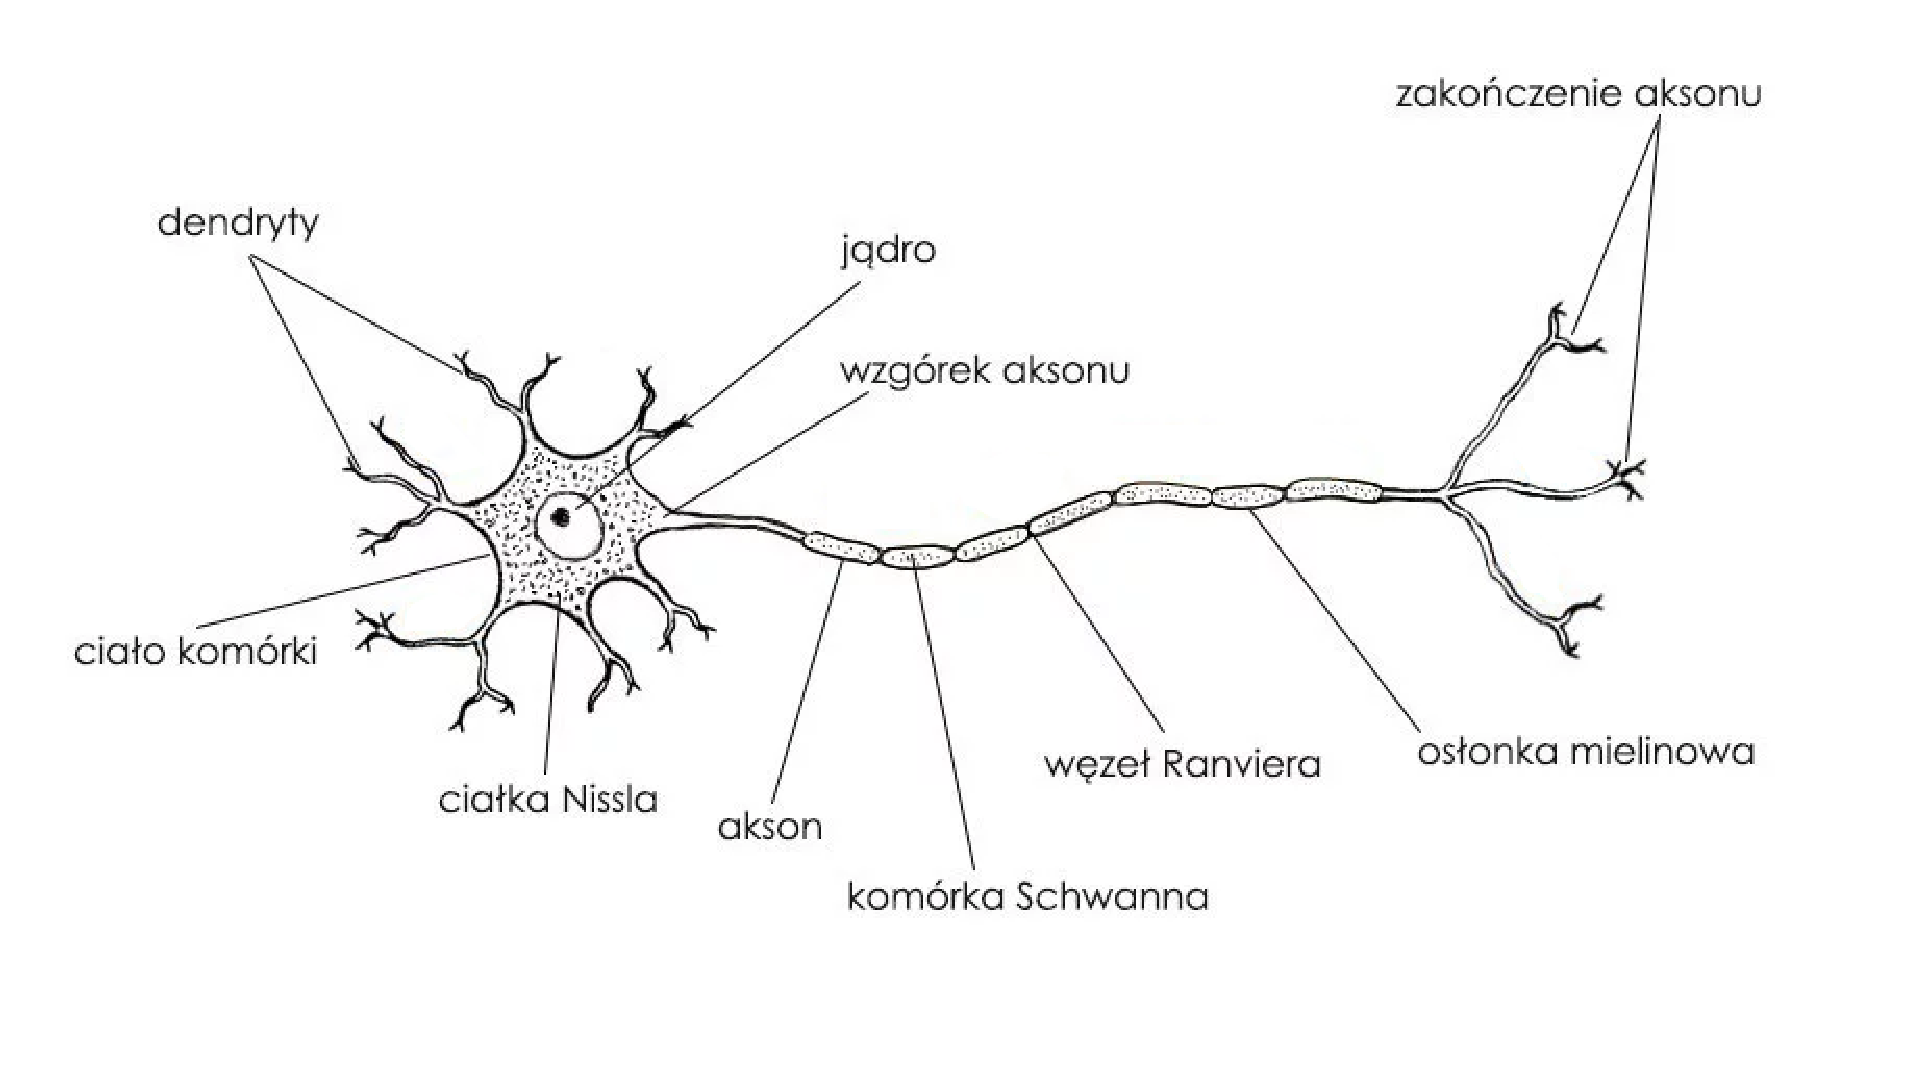
\includegraphics[width=\textwidth]{figures/neuron}
	\caption{Komórka nerwowa \tiny{źródło: www.fizjoterapeuty.pl}}
\end{figure}
Jak pokazano na rysunku \ref{fig:neuron} w skład komórki nerwowej wchodzą dendryty które zbierają
sygnały i akson który je przekazuje dalej.

\FloatBarrier
%--------------------------------------------------------------------------------------------------
\subsection{Model neuronu jako klasyfikator}

\begin{equation}
	\label{equ:two_point_loc}
	IoU = \frac{|A \cap B|}{|A \cup B|}
\end{equation}
%--------------------------------------------------------------------------------------------------
\subsection{Uczenie sztucznych sieci neuronowych}

%--------------------------------------------------------------------------------------------------
\subsection{Konwolucyjne sieci neuronowe}


%==================================================================================================
\section{Architektura kontowlucyjna w detekcji chorób liścia kukurydzy}

%--------------------------------------------------------------------------------------------------
\subsection{Źródło danych}

%--------------------------------------------------------------------------------------------------
\subsection{Opis eksperymentu}

%--------------------------------------------------------------------------------------------------
\subsection{Rezultaty}

%--------------------------------------------------------------------------------------------------
\subsection{Wnioski}
\nocite{*}
\bibliography{bibliografia} 

\end{document}


